\chapter{\huge Metodo Runge-Kutta}

\textit{In analisi numerica i metodi Runge-Kutta sono una famiglia di metodi iterativi impliciti ed espliciti per la risuluzione approssimata di equazioni differenziali ordinarie (ODE). Il più comune di questi metodi è il cosidetto ``RK4'' o anche Runge-Kutta del quarto ordine.}
\\\\
Sia dato il problema di Cauchy
$$ \dot y = f(t, y), \quad y(t_0) = y_0$$
Si assume che il tempo sia discretizzato in istanti $t_n$ equidistanziati di un intervallo $h$.\\
Il metodo RK4 per questo problema è allora dato dalle seguenti equazioni:
\begin{eqnarray*}
y_{n+1} &=& y_n + \tfrac{1}{6} \left(k_1 + 2k_2 + 2k_3 + k_4 \right)\\
t_{n+1} &=& t_n + h
\end{eqnarray*}
dove $y_{n+1}$ è l'approssimazione RK4 di $y(t_{n+1})$, e
\begin{eqnarray*}
k_1 &=& hf(t_n, y_n),\\
k_2 &=& hf(t_n + \tfrac{1}{2}h , y_n + \tfrac{1}{2} k_1),\\
k_3 &=& hf(t_n + \tfrac{1}{2}h , y_n + \tfrac{1}{2} k_2),\\
k_4 &=& hf(t_n + h , y_n + k_3).
\end{eqnarray*}
Il valore della funzione $y$ all'istante $t_{n+1}$ è uguale quindi al suo valore all'istante $t_n$ incrementato della media ponderata di quattro incrementi $k$, dove ogni incremento è il prodotto della dimensione dell'intervallo $h$ ed una stimata pendenza specificata dalla funzione $f$.
\begin{itemize}
\item $k_1$ è l'incremento basato sulla pendenza di $f$ all'estremo sinistro dell'intervallo, calcolato in $y_n$ (metodo di Eulero);
\item $k_2$ è l'incremento basato sulla pendenza nel punto medio dell'intervallo, calcolato in $y_n+\frac{1}{2}k_1$;
\item $k_3$ è ancora l'incremento basato sulla pendenza nel punto medio, calcolato però in $y_n+\frac{1}{2}k_2$;
\item $k_4$ è l'incremento basato sulla pendenza all'estremo destro dell'intervallo, calcolato in $y_n+k_3$.
\end{itemize}
Si nota dalla formula per $y_{n+1}$ che peso maggiore viene assegnato all'incremento al centro dell'intervallo. Inoltre, se $f=f(t)$, cioè non dipende da $y$, il metodo RK4 si riduce alla regola di integrazione di Simpson.

RK4 è un metodo del quarto ordine e quindi l'errore ad ogni step è dell'ordine di $h^5$, mentre l'errore totale accumulato è dell'ordine di $h^4$.

\section{Simulazione di Sistemi Dinamici}
Per mezzo del metodo RK4 è possibile simulare l'evoluzione di sistemi dinamici, in particolare di quelli non lineari o caotici, le cui soluzioni non sono note analiticamente.

Esempi di sistemi dinamici che presentano comportamenti non lineari sono i sistemi di Lorenz, Rossler, Chua e di Rabinovich-Fabrikant.

\begin{figure}[H]
 \begin{subfigure}[b]{0.5\textwidth}
  \centering
  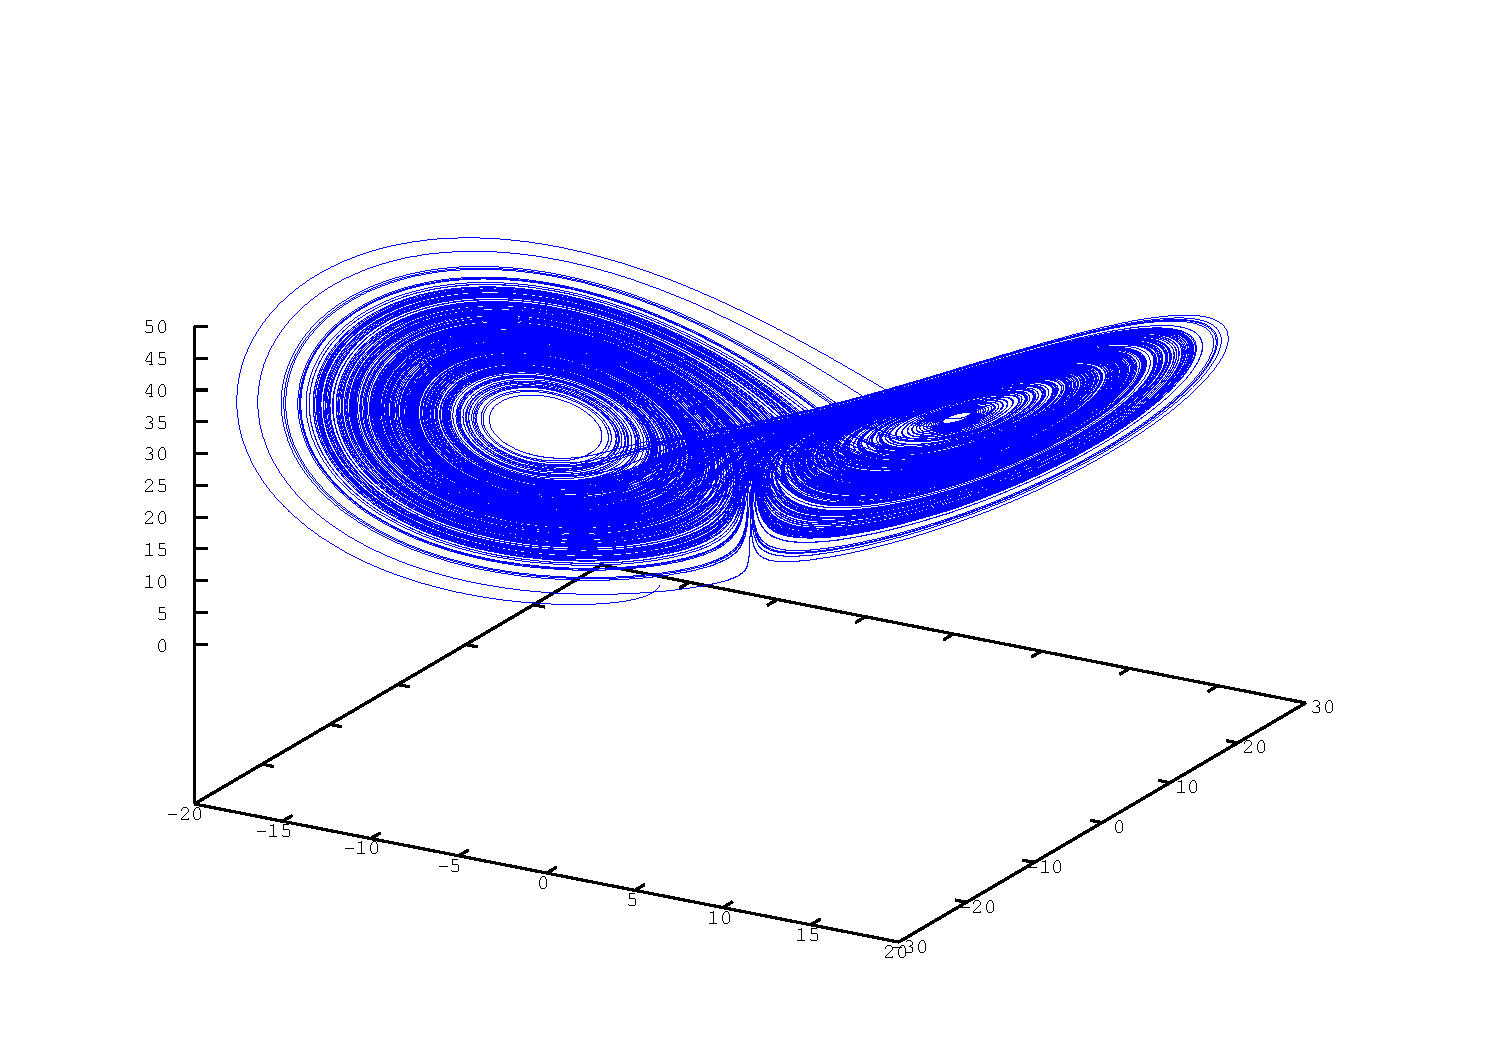
\includegraphics[width=\textwidth]{lorenz}
  \caption{Lorenz}
  \label{fig:lorenz}
 \end{subfigure}
 \begin{subfigure}[b]{0.5\textwidth}
  \centering
  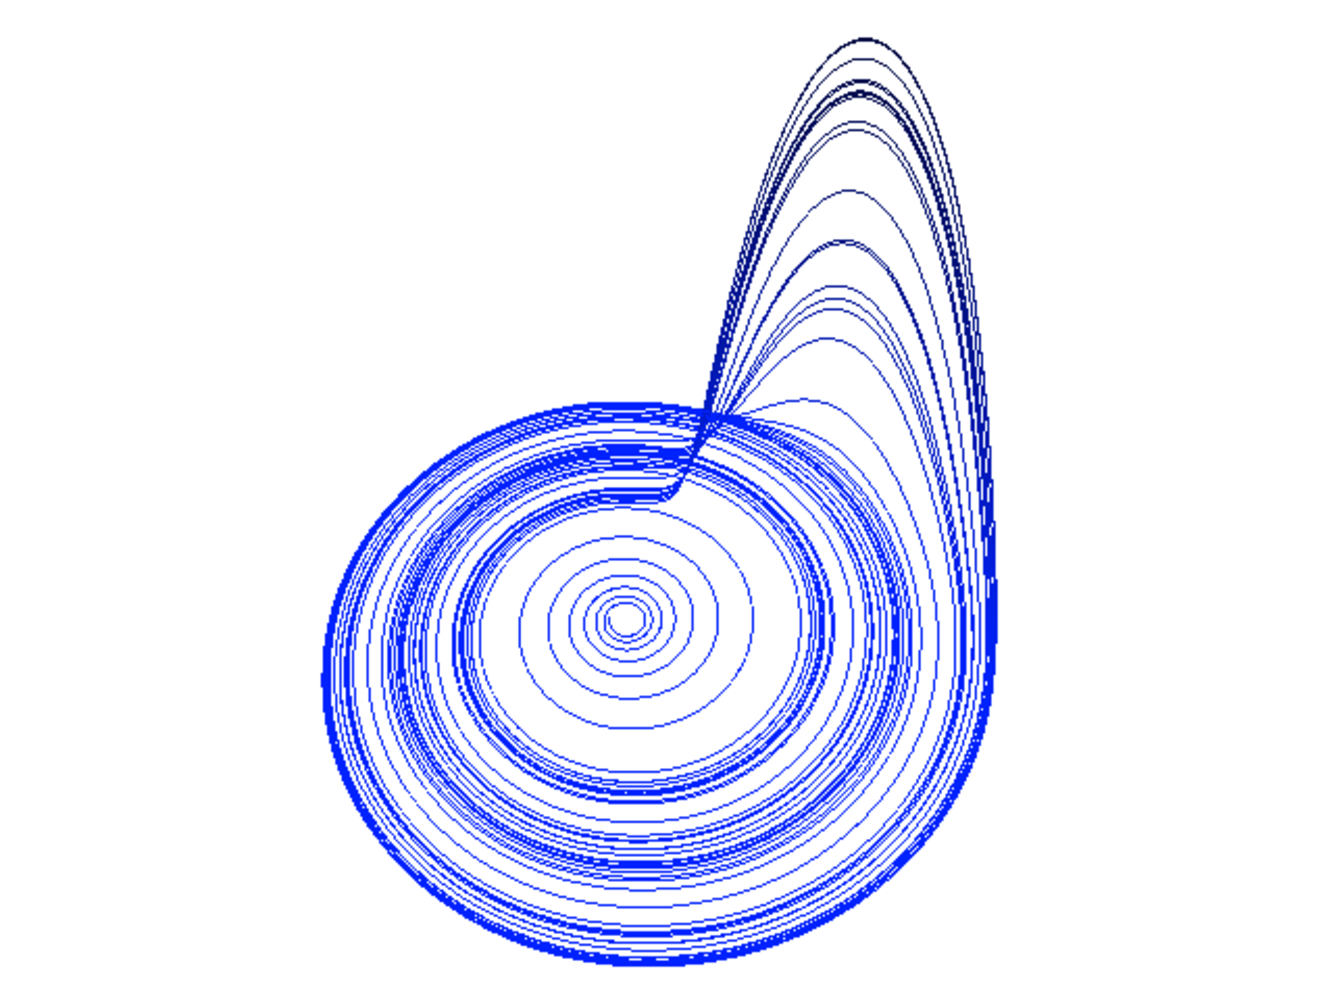
\includegraphics[width=\textwidth]{rossler}
  \caption{Rossler}
  \label{fig:rossler}
 \end{subfigure}

 \quad
 \begin{subfigure}[b]{0.5\textwidth}
  \centering
  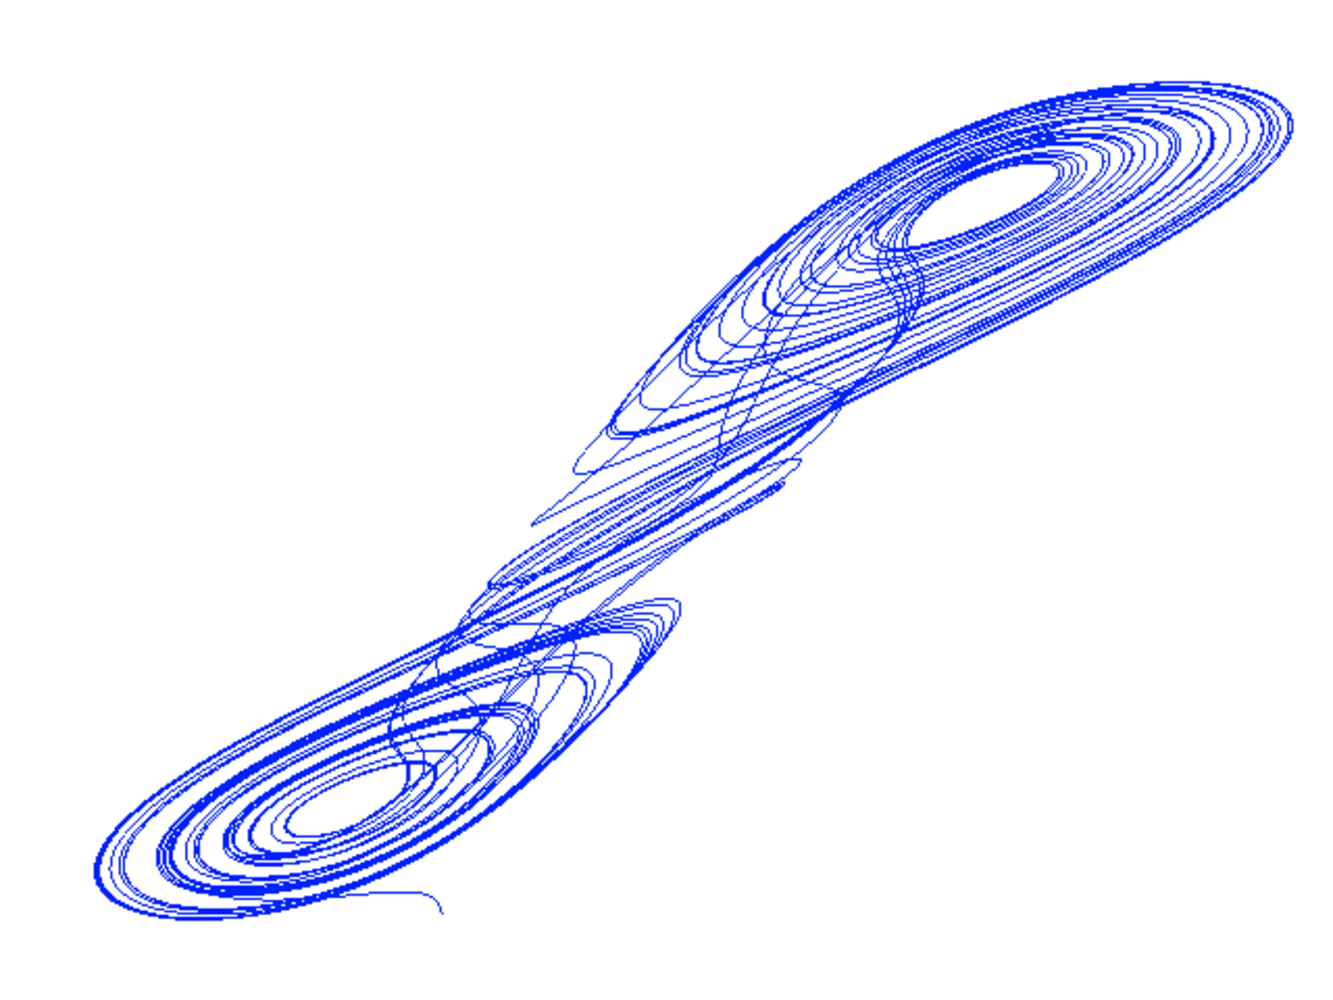
\includegraphics[width=\textwidth]{chua}
  \caption{Chua}
  \label{fig:chua}
 \end{subfigure}
 \begin{subfigure}[b]{0.5\textwidth}
  \centering
  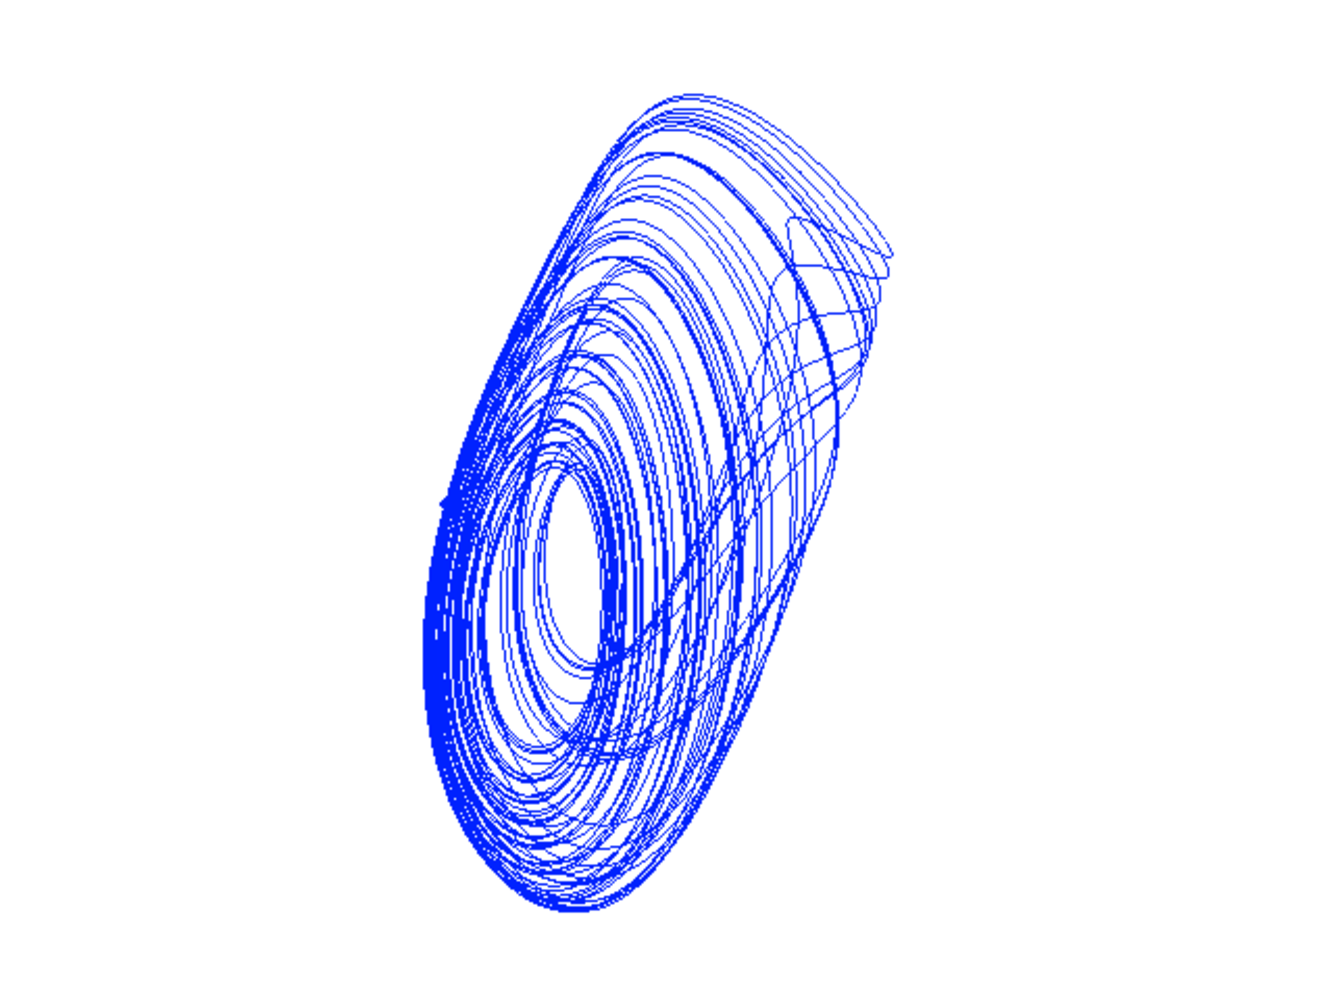
\includegraphics[width=\textwidth]{rf}
  \caption{Rabinovich-Fabrikant}
  \label{fig:rf}
 \end{subfigure}

 \caption{Soluzioni numeriche di sistemi dinamici non lineari}\label{fig:systems}
\end{figure}

La precisione del metodo RK4 decresce considerevolmente con all'aumentare del numero di step della simulazione. L'errore teorico stimato infatti si accumula ad ogni step incrementando la discrepanza con la soluzione esatta. Ciò risulta evidente dal risultato della simulazione rappresentata in figura \ref{fig:rk_error}.

\begin{figure}[H]
\centering
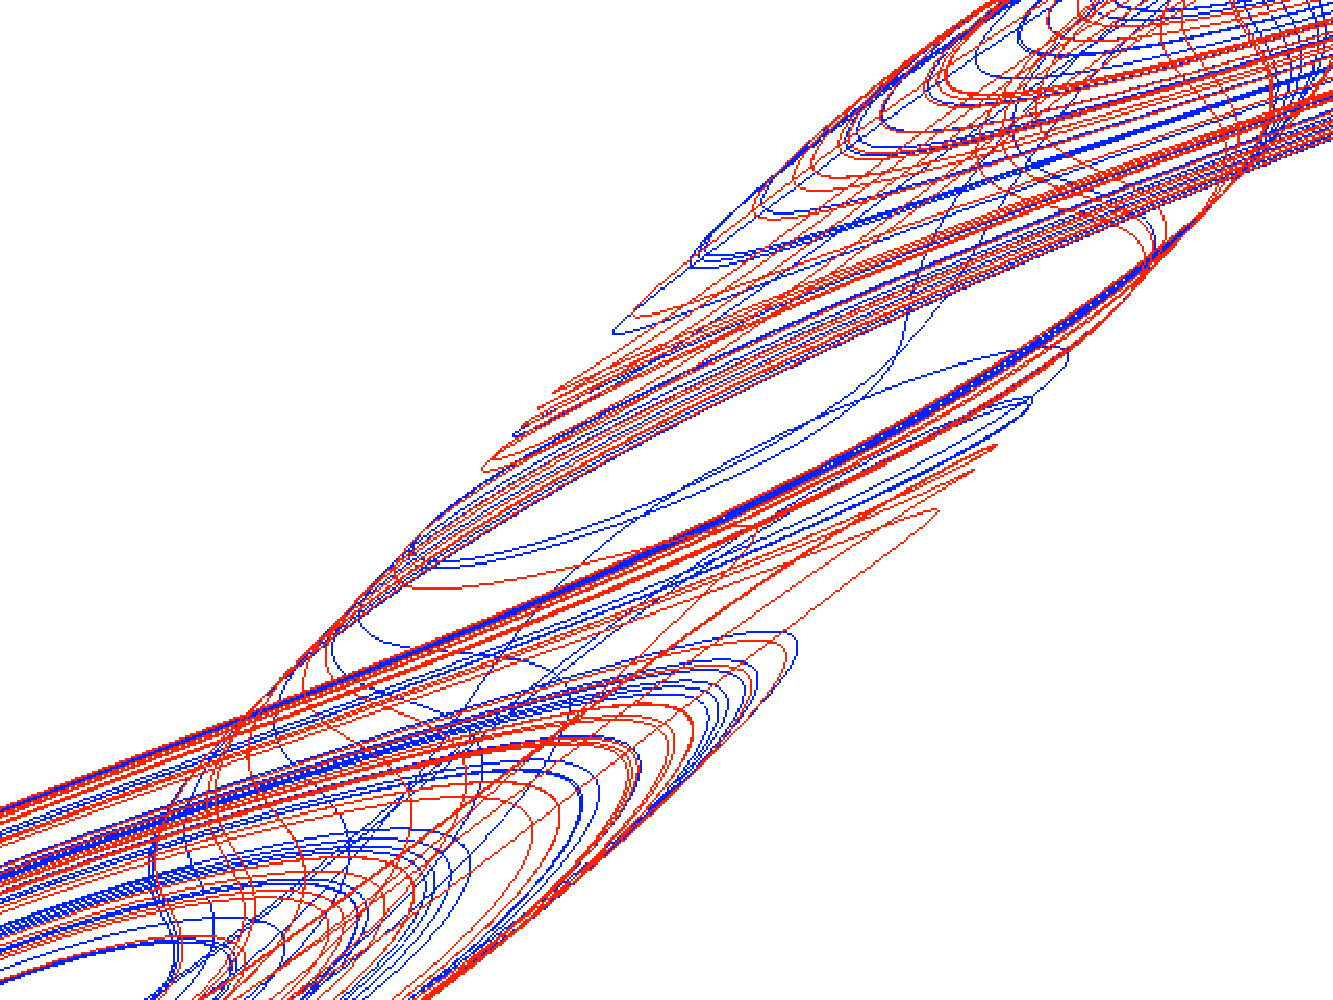
\includegraphics[width=\textwidth]{rk_error}
\caption{Due simulazioni del sistema di Chua con uguali condizioni iniziali e differenti $h$. La linea rossa rappresenta una soluzione numerica calcolata con $h$ doppio rispetto a quello della soluzione in blu.}
\label{fig:rk_error}
\end{figure}

\begin{figure}[H]
\centering
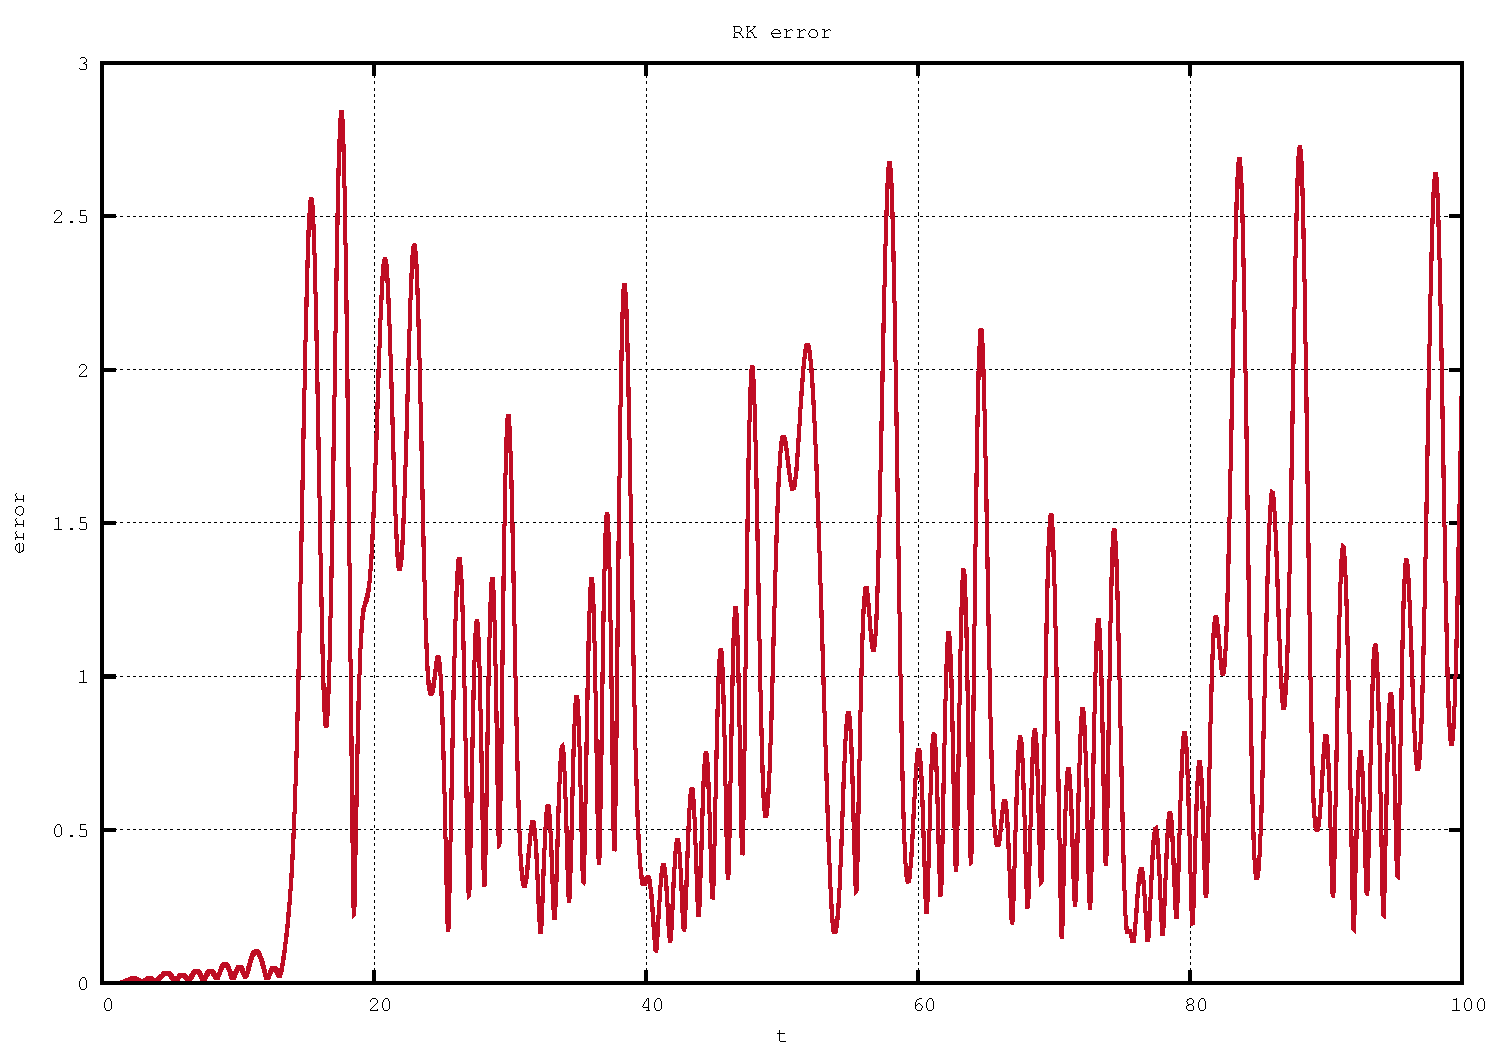
\includegraphics[width=0.6\textwidth]{ode}
\caption{Discrepanza fra le soluzioni in funzione del tempo di simulazione}
\label{fig:ode}
\end{figure}


\subsection{Pendolo Caotico}
Si trovano ora soluzioni numeriche di un sistema non lineare e se ne studia il comportamento al variare dei suoi parametri.
\\

L'equazione del moto di un pendolo non lineare forzato e caotico è:
$$\ddot{\theta}(t) = -\sin(\theta(t)) - q\dot{\theta}(t) + b\cos(\omega t)$$
È possibile ricondurre l'equazione precedente ad un sistema di equazioni differenziali del primo ordine effettuando la sostituzione $x=\theta$, $y=\dot{\theta}$ :
\[
  \Rightarrow \left\{
  \begin{array}{l l}
    \dot{x}=y\\
    \dot{y}=-\sin(x) - qy + b\cos(\omega t)\\
  \end{array} \right.
\]

Applicando ora il metodo RK4 si ottengono le seguenti formule per l'evoluzione delle variabili dinamiche $x,y$
$$x_{n+1}=x_n+hy_n$$
$$y_{n+1}=y_n+\tfrac16 k_{y,1}+\tfrac13 k_{y,2}+\tfrac13 k_{y,3}+\tfrac16k_{y,4}$$
dove i $k_{y,i}$ sono i coefficienti definiti nel paragrafo iniziale e relativi alla seconda equazione del sistema. È facile verificare, invece, che i coefficienti $k_{x,i}$ sono banalmente tutti uguali a $hy_n$, dal momento che $\frac{\partial\dot{x}}{\partial x}=0$.
\\

Di seguito sono raffigurate le traiettorie nello spazio delle fasi $(x,y)$ dell'oscillatore di alcune soluzioni, con uguali condizioni iniziali e $h=10^{-3}$.
\begin{figure}[H]
\centering
\includegraphics[width=0.6\textwidth]{ode1}
\caption{Soluzione per $q=0.3$, $b=0.1$, $\omega=2/3$}
\label{fig:ode1}
\end{figure}

\begin{figure}[H]
\centering
\includegraphics[width=0.5\textwidth]{ode2}
\caption{Soluzione per $q=0.3$, $b=0.5$, $\omega=2/3$}
\label{fig:ode2}
\end{figure}

\begin{figure}[H]
\centering
\includegraphics[width=0.5\textwidth]{ode3}
\caption{Soluzione per $q=0.3$, $b=0.9$, $\omega=2/3$}
\label{fig:ode3}
\end{figure}

\begin{figure}[H]
\centering
\includegraphics[width=0.5\textwidth]{ode4}
\caption{Soluzione per $q=0.3$, $b=1.4$, $\omega=2/3$}
\label{fig:ode4}
\end{figure}

Quello che si nota è che il sistema presenta in tutti e quattro i casi un ciclo limite. Aumentando di poco l'intensità della forzante aumentano anche le dimensioni di tale curva. Quando però $b$ diviene troppo grande, come nel terzo e quarto caso (fig.\ref{fig:ode3}, \ref{fig:ode4}), il ciclo limite assume una topologia totalmente differente dai casi precedenti.
